\section{Aufbau}
\label{sec:Durchführung}

Der Versuchsaufbau ist in Grafik \ref{Aufbau} abgebildet. Als $\gamma$-Quelle dient ein $^{137}$Cs-Strahler, welcher in einer Bleihalterung eingebaut wird. Durch eine kleine Öffnung in der Abdeckung wird ein Strahl kollimiert. Dieser trifft auf einen 3x3x3 cm großen Würfel, der aus 3x3x3 kleineren Würfel zusammengesetzt ist. Die Würfel besitzen damit eine Kantenlänge von jeweils 1 cm.
 Die Probenhalterung auf den der Würfel befestigt wird, erlaubt es den Würfel um seine z-Achse zu drehen, sowie ihn im Strahl zu verschieben. 
 Bei Durchlaufen des Würfels wird der Strahl abgeschwächt und fällt in den NaJ-Detektor. Dort wird mithilfe der Auswertungselektronik ein Histogramm der einfallenden Energien erzeugt.
 Zur Messung stehen mehrere Würfel bereit. Würfel 1 ist ein leerer Würfel nur aus den Aluminiumgehäuse, welchen alle Würfel umgibt. Würfel 2 und 3 bestehen aus jeweils einen zu bestimmenden Material. Würfel 4 ist eine Zusammensetzung aus den Materialien aus denen Würfel 2 und 3 bestehen.

 \begin{figure}
    \centering
    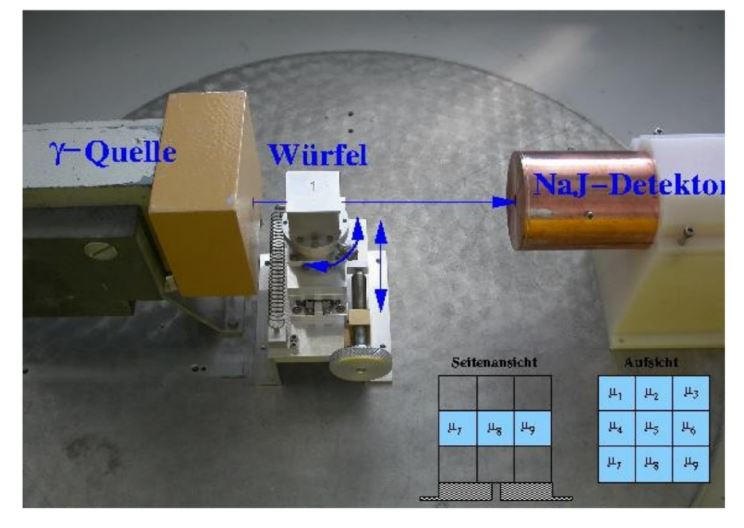
\includegraphics[width=0.9\textwidth]{content/aufbau.JPG}
    \caption{Versuchsaufbau und schematische Zusammensetzung der Würfel. Aus Strahlenschutzgründen wurde dieser Aufbau zusätzlich mit Bleiblöcken abgeschirmt. \cite{Anleitung}}
    \label{fig:Aufbau1}
  \end{figure}

\section{Durchführung}

Um alle Würfel bestimmen zu können sind mindestens 9 Messungen nötig. Um mögliche Messungenauigkeiten ausgleichen zu können werden aber mehr Messungen durchgeführt. Die gewählten Projektionen sind in Abbildung \ref{projektion} dargestellt. 
Zuerst wird der Intensitätsabfall durch die Aluminiumhülle ausgemessen. Dafür wurde jeweils eine Projektion gerade durch den Würfel, mittig queer durch den Würfel, und um einen Elementarwürfel versetzt durch den Würfel aufgenommen. Damit wurde das $I_0$ aller anderen Projektionen bestimmt.
Bei den Würfeln 2 und 3 wurden diese Projektionen ebenso aufgenommen. Da die Würfel aus homogenen Material sind, reicht diese Anzahl an Projektionen aus um das Material der Würfel zu bestimmen.
Bei den zusammengesetzten Würfel 4 wurden alle eingezeichneten Projektionen aufgenommen.

\begin{figure}
    \centering
    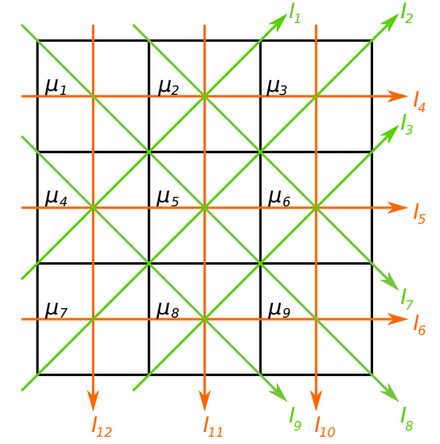
\includegraphics[width=0.9\textwidth]{content/projektion.JPG}
    \caption{Gewählte Projektionen der Messung}
    \label{fig:Aufbau2}
  \end{figure}

